\hypertarget{semaine-haute-en-couleurs-au-puxe9rou}{%
\section{Semaine haute en couleurs au Pérou
!}\label{semaine-haute-en-couleurs-au-puxe9rou}}

\emph{Mardi 11 septembre 2018}

Après un bus de nuit depuis San Pedro de Atacama, on traverse pour la
première fois du voyage une frontière terrestre, entre Arica (Chili) et
Tacna (Pérou). Sur ce long trajet (près de 20 heures) qui nous mène
jusqu'à Arequipa, nous découvrons les joies de ces trajets en bus longue
distance tant vantés par les voyageurs d'aujourd'hui. Après un San
Pedro-Arica plutôt confortable dans nos sièges inclinables avec petit
snack à bord, c'est ensuite que commence l'immersion. Alpagués de
partout, notre trajet péruvien sera très local : arrêts fréquents pour
prendre des voyageurs en stop sur le bord de la route, mais aussi les
différents vendeurs de nourriture, médicaments qui guérissent tout avec
petit discours pseudo-scientifique (si vous êtes fatigués/si vous
baillez/si votre enfant mange des sucreries/si vous transpirez/si vous
avez des gaz : ce sont les parasites ! Prenez-donc de ce super produit
qui va guérir toute la famille), le film de guerre avec volume à fond...
L'expérience est rigolote, mais finalement on ne regrette pas d'avoir
abandonné notre plan initial, qui était de parcourir toute la côte ouest
de l'Amérique du Sud en bus (soit 120 heures de voyage).

Notre programme au Pérou sera le suivant : découvrir Arequipa, se rendre
à Cusco d'où on partira en excursion jusqu'au village inca du Machu
Picchu et finir notre séjour à Lima, la capitale. Voici la carte :

\begin{figure}
\centering
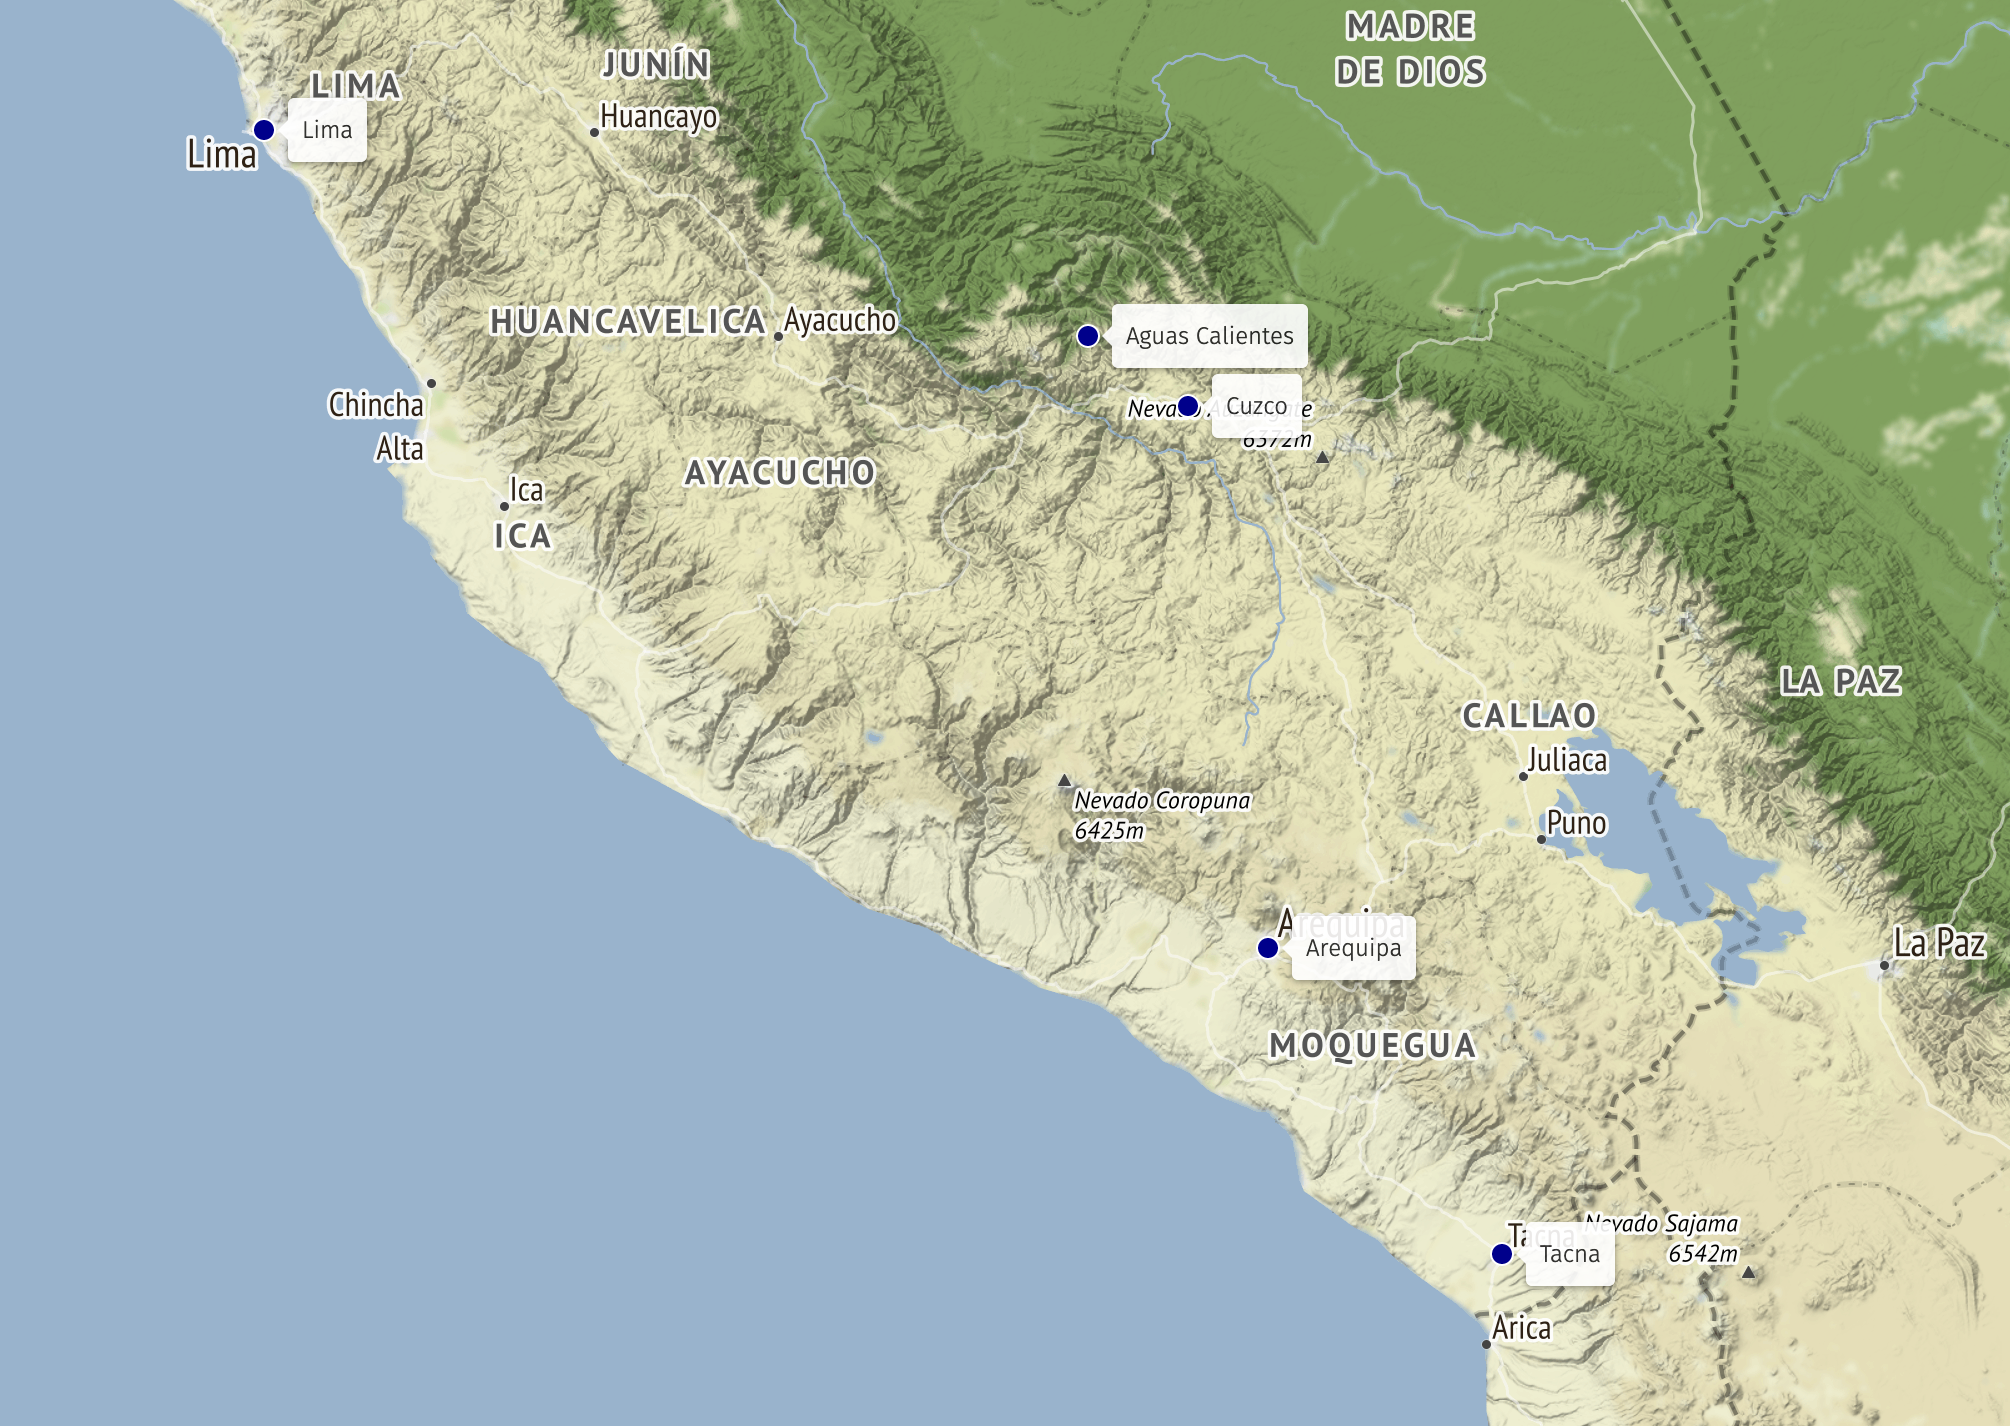
\includegraphics{maps/Peru.png}
\end{figure}

\hypertarget{arequipa}{%
\subsection{Arequipa}\label{arequipa}}

Nos premiers pas au Pérou nous mènent à travers la belle ville
d'Arequipa, avec son agréable place d'Armes et ses bâtiments blancs
datant de l'époque coloniale.

\begin{figure}
\centering
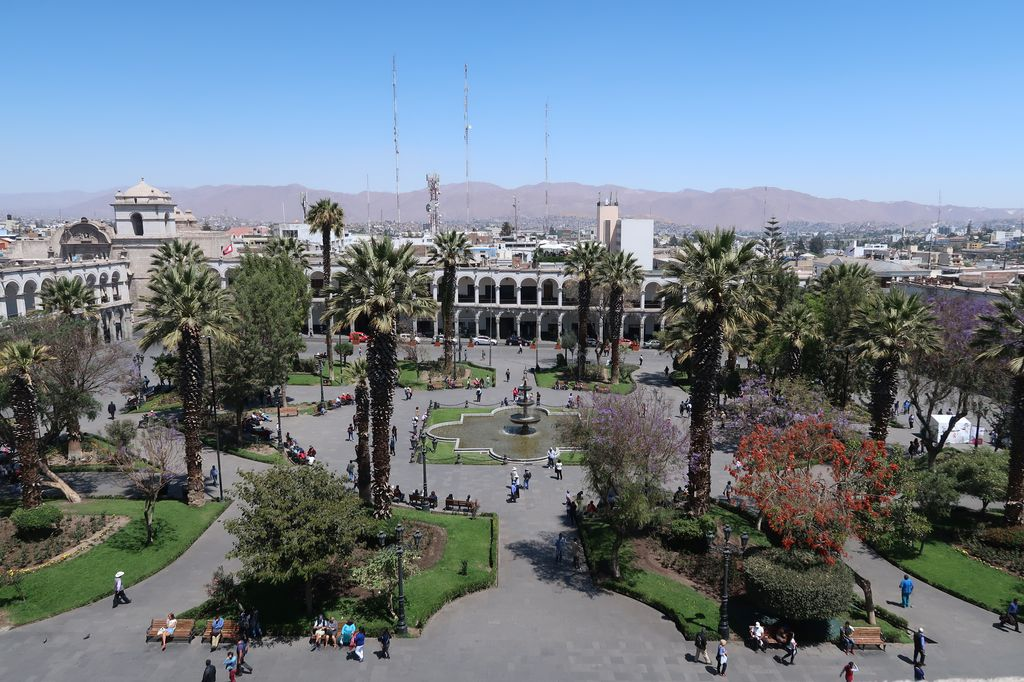
\includegraphics{images/20180911_arequipa.JPG}
\caption{Arequipa.}
\end{figure}

Ayant bien aimé le \emph{free walking tour} qu'on avait testé à Santiago
(tour guidé basé sur les pourboires), c'est comme ça qu'on a commencé à
explorer la ville. Malheureusement les tours ne se valent pas tous, et
c'est avec un énorme groupe et un guide qui parle beaucoup trop vite et
de manière trop dramatique qu'on a passé l'après-midi. Extrait :

\begin{quote}
quoi? AUCUN d'entre-vous n'est déjà monté à plus de 6000 mètres
d'altitude ?? AAAAAAHHHHH mais c'est pas possible ! AUCUN ??? Mais je
vais sauter par-dessus la rambarde ! VOUS ÊTES SÛRS ???? Je le crois pas
!
\end{quote}

Voilà voilà. On a quand même appris que Arequipa vient d'une phrase
Quechua qui signifie "ok vous pouvez rester là", adressée aux colons
espagnols qui en ont profité pour fonder la ville. On a aussi visité la
Cathédrale (visite guidée obligatoire, mais guide bien moins bavard
cette fois) avec son orgue majestueux et sa terrasse avec vue sur la
ville et ses volcans qui imposent le respect (et pas seulement parce que
le premier est encore très actif) : le Misti, le Picchu Picchu et le
Chachani.

\begin{figure}
\centering
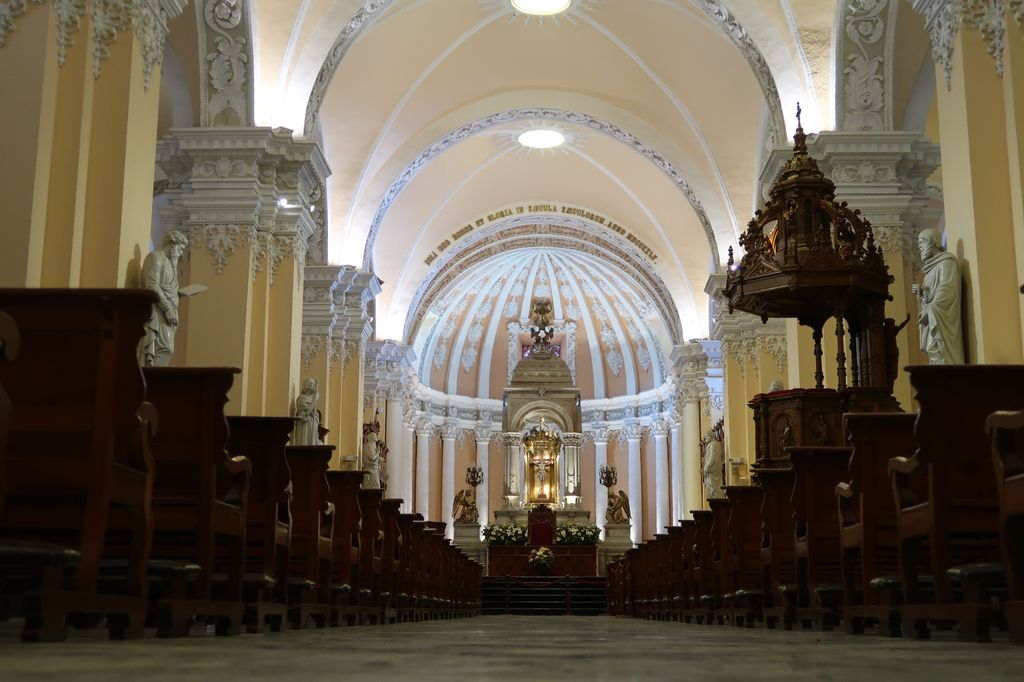
\includegraphics{images/20180911_cathedrale.JPG}
\caption{La cathédrale.}
\end{figure}

Le marché nous en a mis plein la vue avec ses sections colorées et
parfumées, les fruits parfaitement rangés (et malheur sur toi si tu y
touches...), les abats dans tous les sens, les dizaines de types de
pommes de terre différents et les petits stands où on mange plutôt très
très bien ! En parlant de gastronomie, on s'est essayé à des spécialités
locales, notamment les ceviche (qu'on avait déjà apprécié au Chili), la
viande d'alpaca (délicieuse), le cuy (cochon d'Inde grillé : on a testé
mais on a pas adoré..."mais attends, c'est pas les dents ça ? arghhhh"),
la chicha (boisson à base de maïs violet fermenté) et toujours la
boisson nationale créant un conflit avec le Chili : le Pisco Sour. Fun
fact au passage : il est interdit de faire rentrer au Pérou toute
boisson portant la dénomination "Pisco" sur la bouteille ou tout produit
dérivé du Pisco, c'est écrit noir sur blanc aux douanes et ils rigolent
pas avec ça ! Et comme nous avait prévenus notre amie péruvienne Luz
Marina : "le Pisco Sour, ça se boit comme de la limonade, mais ça tape
comme de la vodka !", effectivement !

\begin{figure}
\centering
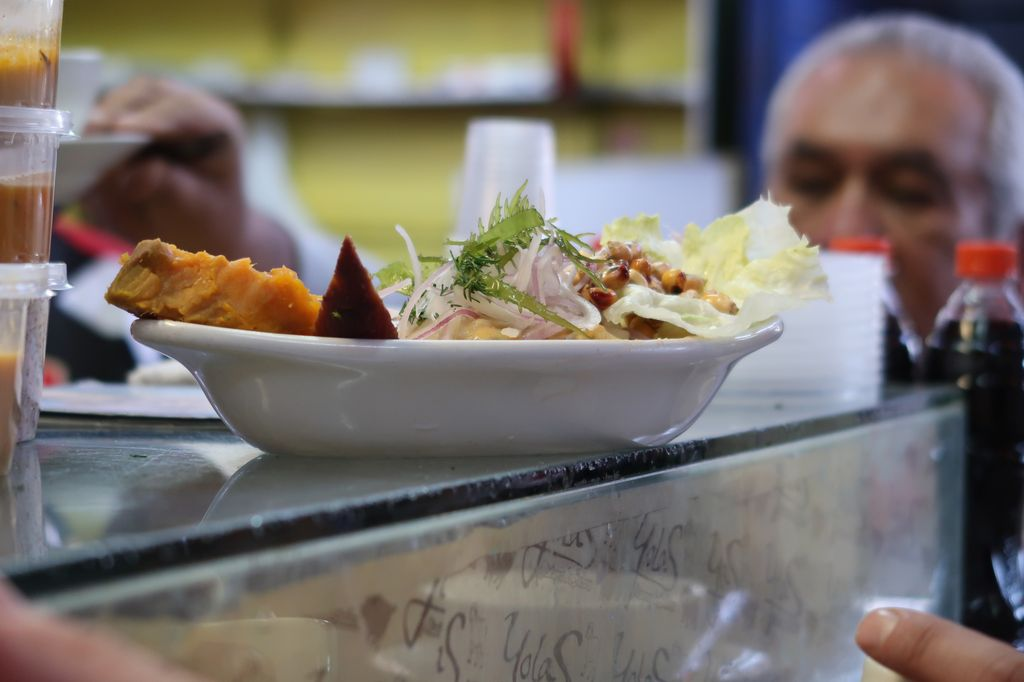
\includegraphics{images/20180911_ceviche.JPG}
\caption{Délicieux ceviche du marché !}
\end{figure}

Mais Arequipa nous a \emph{vraiment} étonné par deux choses. La première
est le très agréable couvent de Santa Catalina, construit par les
espagnols. Une vraie ville dans la ville, avec des maisons, des places,
une fontaine, une laverie. Jusqu'à 400 personnes y ont vécu en même
temps, mais pas que des religieuses : celles-ci avaient chacune une
voire plusieurs servantes ! Aujourd'hui, elles sont une dizaine et
vivent à nouveau en communauté dans un seul et même bâtiment, avec leur
potager, et ont une vie moins luxueuse mais aussi moins cloîtrée que les
prédecesseuses...

\begin{figure}
\centering
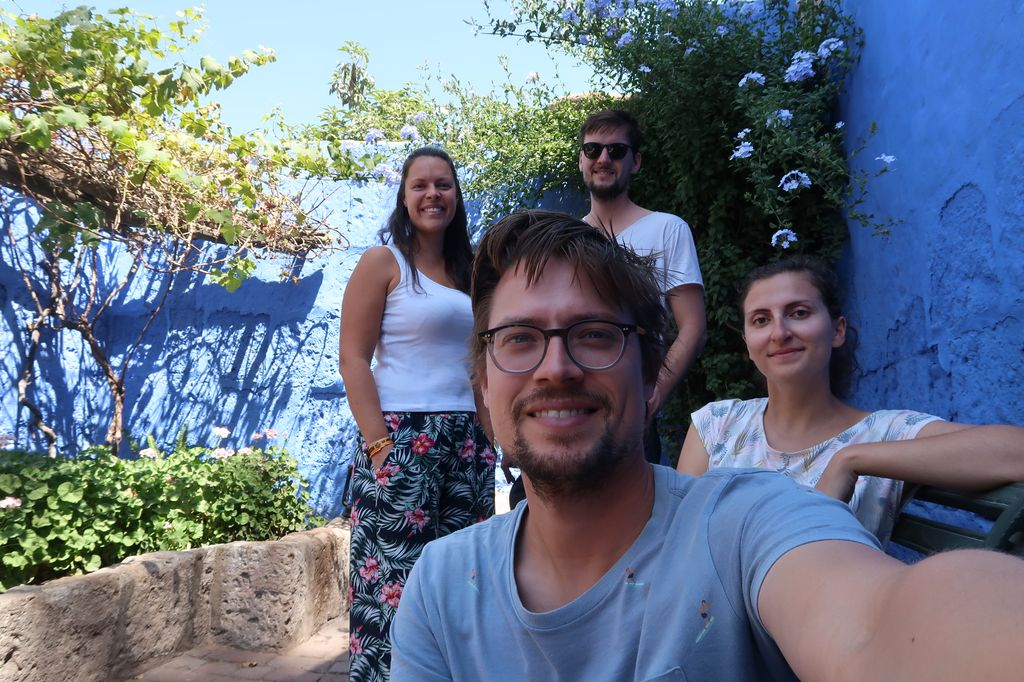
\includegraphics{images/20180911_catalina.JPG}
\caption{Dans le patio d'une des maisons du couvent.}
\end{figure}

La deuxième s'appelle Juanita. Retrouvée momifiée par le froid, cette
jeune adolescente a été sacrifiée par les Incas dans les hautes Andes,
sans doute pour apaiser le dieu du soleil, Inti, et faire cesser les
éruptions volcaniques dans la région. Elle témoigne, à travers son épais
caisson de verre où il fait -18°C, de la tradition des sacrifices
humains chez les Incas, longtemps demeurée incertaine. D'après les
explications du musée, des enfants étaient sélectionnés dès leur
naissance parmi les familles de la haute société pour servir de victime
sacrificielle. Après des jours d'ascension des plus hauts volcans, avec
le matériel de l'époque (sandales aux pieds et manteaux d'alpaca ou de
vigogne), ils étaient assassinés au cours de cérémonies rituelles et
enterrés tout là-haut. C'est sur cette note joyeuse qu'on part pour une
nouvelle aventure en bus de nuit, plutôt confortable, jusqu'à la
capitale des Incas : Cusco.

\hypertarget{machu-picchu-il-faut-le-muxe9riter}{%
\subsection{Machu Picchu : il faut le mériter
!}\label{machu-picchu-il-faut-le-muxe9riter}}

En arrivant le matin à Cusco, on a quelques heures avant notre long
trajet pour le Machu Picchu. Notre taxi, señor Willy, a une proposition
plus intéressante que notre projet initial de traîner dans un café sur
la place d'Armes : il nous emmène de bon matin au site inca de
Sacsayhuaman, sur les hauteurs de Cusco, dont nous n'avions pas du tout
connaissance de l'existence... Équipés de notre pass touristique (qu'on
utilisera à maintes reprises malgré notre court séjour à Cusco), on
visite ce très grand et impressionnant site, avec une vue panoramique
sur la ville et toutes les collines environnantes.

\begin{figure}
\centering
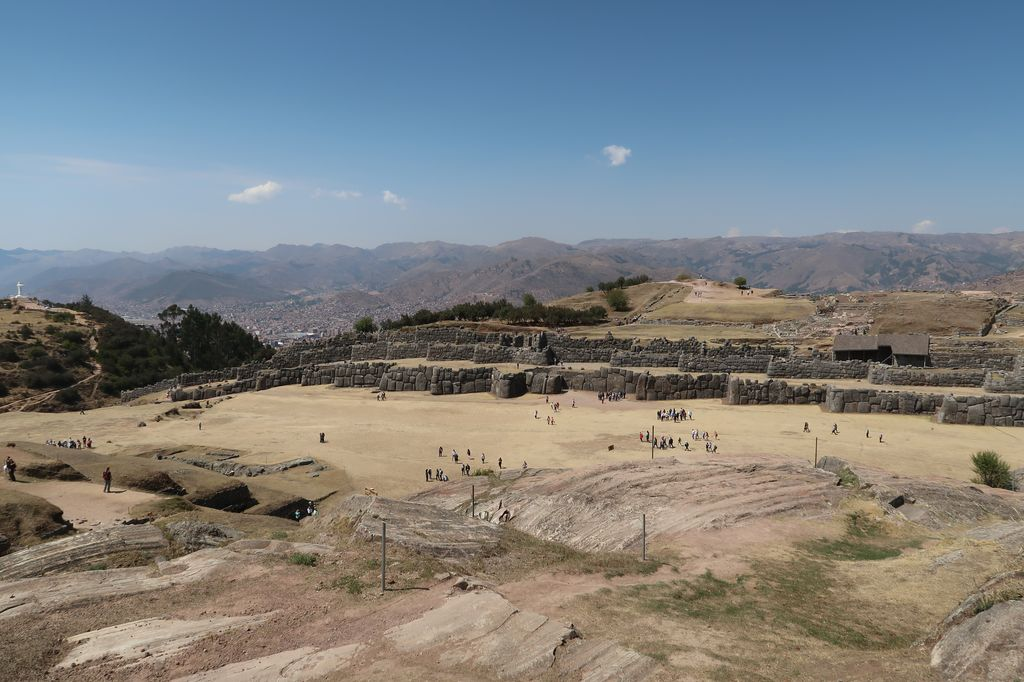
\includegraphics{images/20180911_cusco_sacsaywoman.JPG}
\caption{L'immense site de Sacsayhuaman.}
\end{figure}

On prend ensuite un taxi pour Ollantaytambo d'où part notre train pour
Aguas Calientes, au pied du Machu Picchu. Notre chauffeur nous propose
aussi un arrêt culturel sur le chemin, à Chinchero, où se trouvent des
terrasses incas impressionnantes et un charmant village en pleine
ébullition : il se prépare la fête de la "Virgen Natividad", et tout le
monde met la main à la pâte pour préparer de grands chars portatifs
décorés de mille couleurs avec des statues ou des images de la Vierge.
Arrivés à Ollantaytambo, on profite des quelques heures qui nous restent
avant le train pour attraper une empanada et explorer de nouvelles
ruines incas, faites de terrasses et de temples. Pour l'instant,
l'histoire de ces villages incas nous échappe, car les panneaux
explicatifs sur place sont...inexistants ! Mais on garde toutes nos
interrogations sous le coude, pour le premier guide qu'on croisera...

\begin{figure}
\centering
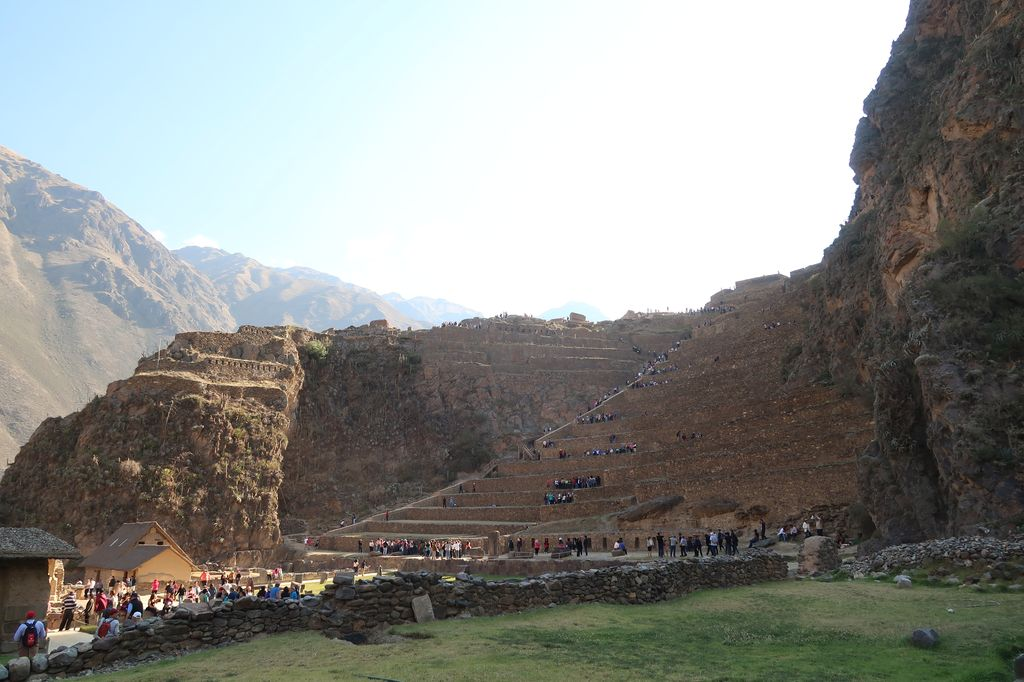
\includegraphics{images/20180911_ollantaytambo.JPG}
\caption{Une partie du site impressionnant d'Ollantaytambo.}
\end{figure}

La dernière partie de cette grosse journée se passe dans le train entre
Ollantaytambo et Aguas Calientes, d'où on partira à pied pour le Machu
Picchu. C'est à Raphaël qu'on a confié la mission d'organiser ces deux
jours, et ça a été un vrai casse-tête ! Qui aurait dit qu'il fallait une
demi-journée pour parcourir les 60 kilomètres qui relient Cusco à Aguas
Calientes ? Vu le peu de temps qu'on avait pour le Pérou, le train,
malgré son prix bien élevé, était la solution la plus rapide pour
nous... Et plutôt agréable : les paysages qu'on a traversés étaient
magnifiques, sur fond de musique traditionnelle.

A Aguas Calientes, on s'installe dans notre sympathique auberge de
jeunesse et on se met vite en recherche d'un endroit pour dîner : il
faut se lever très tôt le lendemain ! C'est à 4h30 du matin qu'on se met
en marche. Au pied de la montagne, on passe le contrôle des billets à un
peu avant 5h30, puis on attaque la montée à pieds. Une grosse heure
d'escaliers plus tard, on arrive enfin au site. La magie opère, on se
retrouve face à la vue qu'on connaît du village inca !

\begin{figure}
\centering
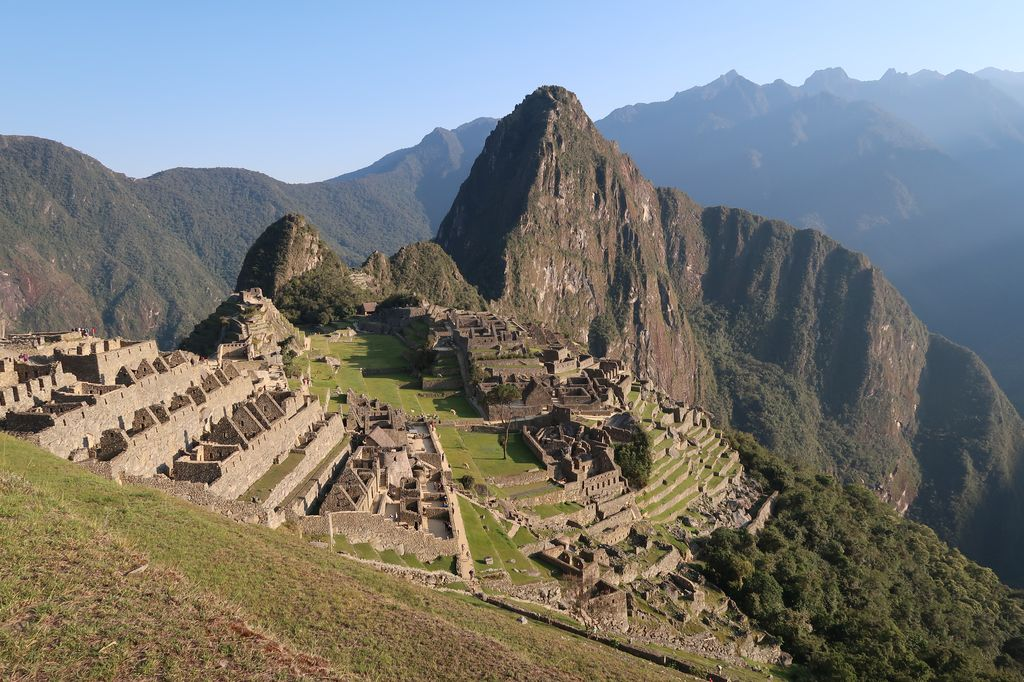
\includegraphics{images/20180911_machupicchu.JPG}
\caption{Le seul et unique.}
\end{figure}

Mais déjà il faut continuer à grimper : on a un billet pour la montagne
Picchu, qu'il faut qu'on commence à monter avant 8 heures ! C'est deux
heures et 2670 marches plus tard (j'ai arrêté de compter à 1300, ça
devenait de plus en plus sportif et raide \^{}\^{}) qu'on arrive à 1000
mètres de dénivelé de notre point de départ, au sommet de la montagne
Picchu, où on a une vue panoramique à couper le souffle. On est entourés
de montagnes aux sommets enneigés, d'un côté de la vallée on aperçoit un
cours d'eau qui nous fait réaliser tout ce qu'on a grimpé, de l'autre
côté la vue dont on ne se lasse pas, de ce village qui nous est encore
mystérieux... Après un pique nique qu'on savoure, on envisage avec
appréhension la descente sur nos jambes bien fatiguées. Arrivés au
niveau du site, on se lance dans deux heures de visite guidée qui
permettront de lever le voile sur un certain nombre de nos
interrogations. Le Machu Picchu ne peut pas être qualifié de ruines
parce que 80\% du village est resté intact, avec seulement les toits en
moins... Le village aurait été abandonné par les incas qui ont détruit
le sentier qui y accède (le fameux inca trail, qui se randonne en 4
jours) afin que le lieu reste secret. Et ça n'a pas raté, il a été
oublié pendant 350 ans, faute de trace écrite de son existence. Enfin
pas complètement, car on a appris que deux familles de paysans ont pris
possession du lieu et y vivaient quand il a été redécouvert par Hiram
Bingham en 1911 et révélé aux yeux du monde...

\begin{figure}
\centering
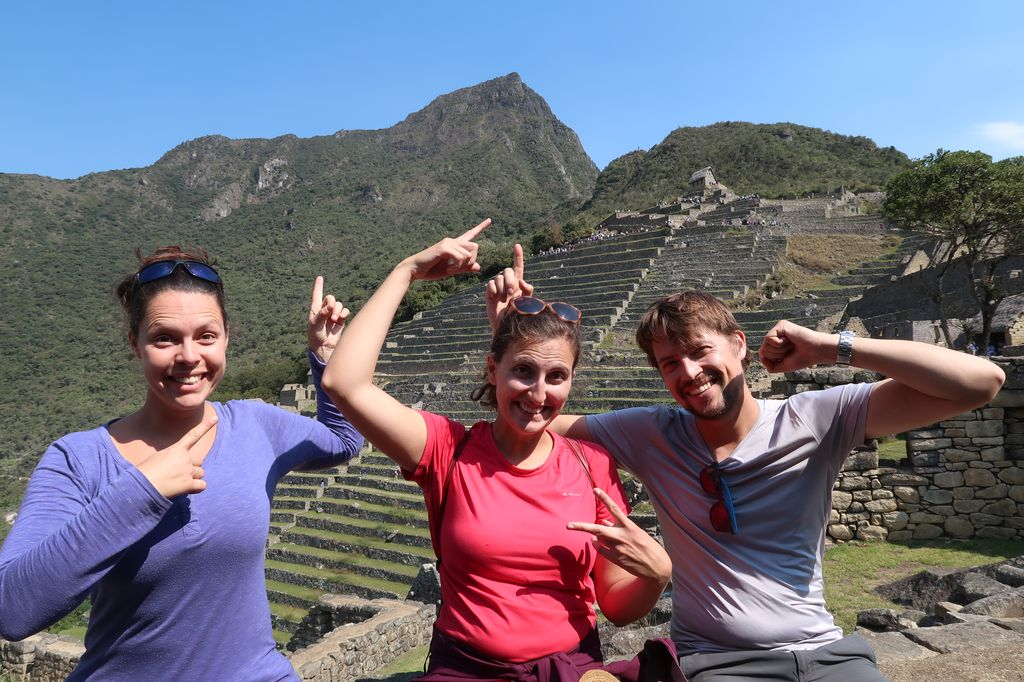
\includegraphics{images/20180911_montana.JPG}
\caption{C'est tout là-haut qu'on était quelques heures plus tôt !}
\end{figure}

On y découvre aussi l'ingénieux système de terrasses qui permet de
cultiver différentes espèces dans des microclimats différents à chaque
étage, l'entier système d'évacuation des eaux de pluie qui a tellement
bien fait son travail qu'il a permis d'éviter l'éboulement du site
pendant plusieurs centaines d'années, et le système des fontaines qui
récupérait l'eau d'une source plutôt éloignée pour l'acheminer au cœur
du village. Jusqu'à 600 personnes auraient vécu sur le site, que ce soit
l'Inca (le roi) et sa famille en résidence d'été ou les ouvriers qui
payaient leur taxe en travaillant 4 mois par an pour le "gouvernement".
Tout a été construit en fonction du soleil, et le temple d'Inti (le dieu
du soleil, pour ceux qui suivent pas) est baigné de lumière au moment du
solstice d'été. On se lance enfin dans la descente finale, qui nous
ramène à Aguas Calientes où on attrape notre train retour pour Cusco.
L'agréable surprise du surclassement en première classe, avec Pisco, vin
à volonté et délicieux repas complet n'aura rien gâché à une journée
déjà merveilleuse ! On gardera un souvenir ému du Machu Picchu, et nos
jambes ne manqueront pas les jours suivants à nous rappeler nos
exploits.

\hypertarget{cusco}{%
\subsection{Cusco}\label{cusco}}

C'est en arrivant à Cusco qu'on réalise que notre programme est encore
plus serré qu'on le pensait. On n'a qu'une journée complète pour
découvrir la capitale des Incas, avec les courbatures de la veille en
prime ! On fait donc appel à señor Willy qui nous envoie son fils en
guise de taxi. On visite les sites incas de Qenqo (lieu de culte et de
rites), Pukapukara (forteresse militaire) et Tambomachay (lieu de
fontaines), puis le musée de Qoricancha où on apprendra des choses
intéressantes et pas du tout sanglantes sur les pratiques de trépanation
et de déformation des crânes chez les incas, sympa ! On y recroise même
une momie, un peu moins fraîche que Juanita...

\begin{figure}
\centering
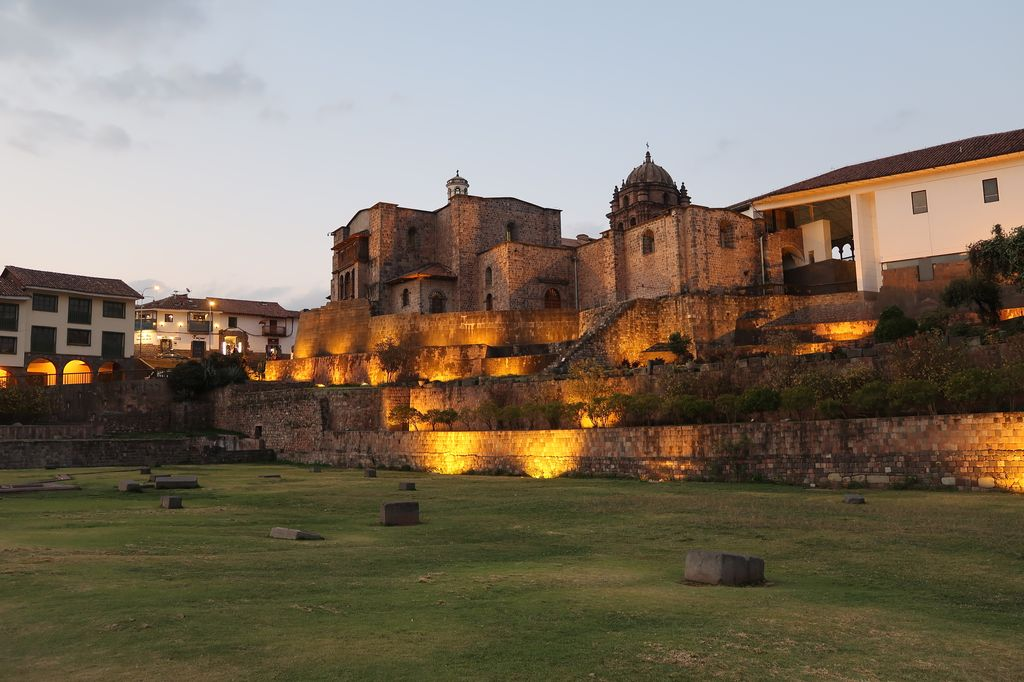
\includegraphics{images/20180911_qoricancha.JPG}
\caption{Fin du jour sur Qoricancha.}
\end{figure}

On ne verra malheureusement le centre ville qu'en coup de vent, mais
l'enchaînement des belles places fait son petit effet. On finit la
journée en beauté par un spectacle traditionnel péruvien (toujours
inclus dans le billet touristique, ça vaut le coup !), avec des musiques
rythmées et des tourbillons de rubans colorés... Nous retrouvons une
dernière fois señor Willy qui nous emmène à l'aéroport pour une encore
plus courte escale, à Lima.

\hypertarget{lima}{%
\subsection{Lima}\label{lima}}

On nous avait prévenus, l'intérêt de Lima est bien moins grand que ce
que nous avons pu voir avant. Fidèles à nous-mêmes, c'est par un
\emph{free walking tour} qu'on se lance dans la découverte de la ville.
Richard nous emmène à travers les places et les églises pour nous
raconter l'intéressante histoire du Pérou, de son métissage, de la vie
trépidante des conquistadores qui se sont bien tapés dessus les uns les
autres (trop d'or, ça leur est monté à la tête), de son indépendance et
de la situation complexe actuelle avec l'accueil de milliers de
vénézuéliens.

Et c'est encore l'heure de partir pour un autre pays. On quitte le Pérou
avec de nombreux souvenirs inoubliables et le ventre bien rempli, mais
aussi avec un regret : celui de ne pas avoir eu plus de temps dans ce
pays. On aurait adoré ajouter au programme les lignes de Nazca, le
canyon de Colca, la montagne des 7 couleurs, ou encore le lac
Titicaca... Une certitude : on reviendra !

\emph{Elida}

\hypertarget{commentaires}{%
\subsection{Commentaires}\label{commentaires}}

\begin{itemize}
\item
  Thibaud, \emph{2018-10-02 17h34}

  Je vois qu'on a photographié les verres de vin vides ! Difficile à
  croire :)
\item
  Florian LB, \emph{2018-10-04 07h16}

  Sans doute une erreur de timing pour la photo ;-)
\item
  pythux, \emph{2018-10-09 19h56}

  Chili en verlant ça fait Lichi...
\item
  Florian LB, \emph{2018-10-12 19h58}

  Ça non plus on en a pas vus beaucoup.
\item
  pythux, \emph{2018-10-09 19h56}

  C'est étrange, je me serais attendu à voir une Synagogue à Arquipa !
\item
  Florian LB, \emph{2018-10-12 19h57}

  Et pourtant on en a pas vue.
\item
  pythux, \emph{2018-10-09 19h57}

  Lorsque vous reviendrez, n'oubliez pas de traverser le Titicaca en
  Tutu kaki !
\item
  Florian LB, \emph{2018-10-12 19h55}

  Ça faisait partie des plans initiaux mais on était à court de temps
  :-(
\end{itemize}


